\chapter{System Architecture}\label{system-architecture}

The architecture presented in this chapter is strictly constraint-driven. Each research question sets a requirement the system has to meet, each requirement forces a design decision, and each decision is later put to a specific test. Table~\ref{tab:rq-design} states those chains up front, so the rest of the chapter can be read as the argument for the middle column, and Chapter 5 as the verdict on the right. The layers that follow develop that argument, and where one of them answers squarely to a single research question it is noted at the head of the section.

% Add this right before your table
\renewcommand{\arraystretch}{1.5} 

\begin{longtable}{@{}
  >{\raggedright\arraybackslash}p{\dimexpr 0.08\linewidth - 1.6\tabcolsep \relax}
  >{\raggedright\arraybackslash}p{\dimexpr 0.30\linewidth - 1.6\tabcolsep \relax}
  >{\raggedright\arraybackslash}p{\dimexpr 0.37\linewidth - 1.6\tabcolsep \relax}
  >{\raggedright\arraybackslash}p{\dimexpr 0.25\linewidth - 1.6\tabcolsep \relax}@{}}
\caption{From research question to design requirement to the architectural choice that meets it, with the section that develops it and the experiment that tests it.}\label{tab:rq-design}\tabularnewline
\toprule
\textbf{RQ} & \textbf{Design requirement} & \textbf{Architectural choice (section)} & \textbf{Tested by} \\
\midrule
\endfirsthead
\toprule
\textbf{RQ} & \textbf{Design requirement} & \textbf{Architectural choice (section)} & \textbf{Tested by} \\
\midrule
\endhead
\bottomrule
\endlastfoot

\textbf{RQ1} & Ingest several platforms through one format, never block the stream, and stay open to extension & One adapter per platform behind a Universal Schema; a durable Kafka log between producers and consumers; storage as the seam so slow work runs off the hot path (Sections~\ref{layer-1-ingestion-and-the-context-agent}, \ref{layer-2-the-streaming-backbone}, \ref{the-universal-schema}) & Latency, throughput, scaling and resource use (Sections~\ref{latency-and-computational-cost}--\ref{throughput-scalability}) \\
\addlinespace[1em] % Forces a distinct physical gap

\textbf{RQ2} & Read context without paying LLM latency on every message & Two tiers split by a confidence gate, with the judge reading its work from storage asynchronously (Sections~\ref{layer-3-two-tier-classification}, \ref{layer-4-storage-and-retrieval}) & Tier-1 against Tier-2 on the same benchmark (Table~\ref{tab:headline}) \\
\addlinespace[1em] % Forces a distinct physical gap

\textbf{RQ3} & Add each kind of context independently, so its effect can be isolated & Context strategies as separate modules feeding one prompt slot, selected by configuration rather than code (Section~\ref{layer-5-context-injection-and-the-analyst-surface}) & One variant at a time, with significance testing (Table~\ref{tab:headline} and Section~\ref{statistical-significance}) \\

\end{longtable}
% Reset arraystretch after the table if needed
\renewcommand{\arraystretch}{1.0}
One decision came early and shaped everything after it, to keep the fast part and add the smart part to it.

A small model can label a message in milliseconds. A large one needs seconds, but understands what it is reading. The pipeline needs both, and there is no single model that is both, so instead of settling for something in the middle the two run in sequence and each does the job it is suited to. Ingestion and first-pass labelling move at stream speed. The expensive reasoning happens off to the side, on a thin slice of the traffic, and its latency never reaches the live path. The system is therefore never blocked by its own intelligence.

Three principles hold the rest of the design together.

\textbf{Decoupling.} Producers never talk to the classifier. They write to a broker, and whatever reads from that broker can change, restart, or scale without the producers noticing. One level up, the same idea repeats: the slow LLM auditor reads from storage instead of sitting in the line, so a slow model cannot slow the stream.

\textbf{Modularity.} Layers speak to each other through fixed contracts, not shared code. A new data source is just another producer emitting the same schema. A new reasoning strategy is just another consumer of the same records. Nothing downstream gets rewritten when something upstream is added, and that is exactly what allows memory, retrieval, and the multi-agent design to be added as separate pieces that can each be measured on their own instead of as edits to one tangled program.

\textbf{Stream-first thinking.} There is no batch pipeline running quietly alongside a real-time one. Data arrives as a stream, is processed as a stream, and is stored so later analysis can query it. Even historical work, re-judging old records or rebuilding the retrieval index, is written as another pass over that same stored stream. This is the Kappa approach, and its practical benefit is that there is only ever one set of logic to keep correct.

\section{The pipeline at a glance}\label{the-pipeline-at-a-glance}

Five layers, each with one responsibility. Figure 3.1 shows the whole path; the sections after it take the layers one at a time.

\begin{figure}[H]
\centering
\includegraphics[width=0.95\linewidth,height=0.85\textheight,keepaspectratio]{figures/arch3.png}
\caption{Five-layer architecture. Storage is the seam of the pipeline: Tier-1 writes every labelled message to Elasticsearch on the hot path, and Tier-2 with its reasoning strategies runs asynchronously off that store rather than inline. The dashed arrows out of storage are those asynchronous reads (the low-confidence sweep and the memory, RAG, and Wiki context lookups); the solid arrows are the live hot path.}
\end{figure}

\begin{enumerate}
\def\labelenumi{\arabic{enumi}.}
\tightlist
\item \textbf{Ingestion and context.} Platform producers pull live messages, and a Context Agent tags each stream with its domain and how strictly it should be moderated.
\item \textbf{Streaming backbone.} Apache Kafka queues the tagged messages; Apache Spark is the distributed processing engine that the design scales out onto.
\item \textbf{Two-tier classification.} A fast DistilBERT model labels every message; uncertain cases are escalated to an LLM judge.
\item \textbf{Storage and retrieval.} Elasticsearch holds every record and its verdicts, Qdrant holds the vectors that power semantic retrieval, and Kibana visualises the stream.
\item \textbf{Context injection and analyst surface.} Temporal memory, retrieval, and the multi-agent decomposition feed the judge; a dashboard and an analyst console sit on top for the humans in the loop.
\end{enumerate}

All five come up from one \texttt{docker-compose} definition. For a Big Data system that matters as much as any design decision, because it makes the architecture something a reader can run rather than only something they can read about.

\section{Layer 1 : Ingestion and the Context Agent}\label{layer-1-ingestion-and-the-context-agent}

Can one pipeline take in several platforms and stay cheap to add to? That is RQ1, and this layer is where it is decided.

Chat arrives messy and platform-specific. This layer turns it into one clean format.

Every platform gets its own producer, called an adapter, and the two used in this thesis were picked partly because they are so unalike. The YouTube adapter polls live chat over HTTP through \texttt{pytchat}. The Twitch adapter holds open an anonymous IRC socket and needs no credentials at all. Different transport, different pacing, different metadata, one output format. That contrast is what gives the multi-platform claim its evidence: the schema had to absorb two genuinely different kinds of source, not two flavours of the same one. Routing between them is trivial. A small script, \texttt{omni\_ingest.py}, reads a pasted URL and hands off to whichever adapter fits, so adding a platform costs one adapter and one line, and nothing else in the system is touched.

Whatever the source be added into the system, everyone of them emits the same \textbf{Universal Schema} (Section~\ref{the-universal-schema}). Downstream code never has to know where a message came from.

There is one more step before a message leaves this layer, and it is the first place the system does something a plain classifier cannot. The \textbf{Context Agent} reads the stream's metadata, its title, its channel, its description, and works out what kind of space this is. Not by picking from a fixed menu, which would turn discovery into guesswork the moment a stream fits nothing on the list, but by describing it in free text and saying how strict moderation ought to be. A gaming stream where ``you're dead'' is ordinary trash talk gets tagged \emph{low} strictness. A political broadcast gets \emph{high}. The free-text answer is then mapped onto a stable taxonomy so the analytics stay consistent, and the model's original wording is kept alongside it, because that wording is data in its own right, a record of the categories the model reached for unprompted. How all this works, and why discovery beats classification here, is Chapter 4's business. What matters architecturally is only this: context is attached at the very edge, before anything else sees the message.

\section{Layer 2 : The streaming backbone}\label{layer-2-the-streaming-backbone}

This is the part of the system grows into the Big Data, using Kafka and Spark.
\textbf{Apache Kafka} is the broker in this design. Producers write to one topic, \texttt{universal\_stream}, and every consumer reads from it at its own pace. Decoupling, made concrete. A viral stream can flood the topic and the classifier just works through the backlog; if the classifier crashes and comes back, Kafka still holds everything it had not yet read. Ordering and fault tolerance come almost free, which a hand-rolled queue would never give. It is deliberately the one component nothing else can bypass.

The deployed settings need stating plainly, because they bound what Chapter 5's throughput numbers can claim. The broker runs as a single node. The topic is created automatically with Kafka's default of one partition and a replication factor of one, and messages are kept for twenty-four hours or one gigabyte, whichever comes first. Partitions are what limit consumer parallelism in Kafka, since a consumer group can have at most as many active consumers as the topic has partitions. With one partition, exactly one Tier-1 process draws from the stream at a time. A single process already sustains far more throughput than the live sources produce (Section~\ref{throughput-scalability}). Raising the ceiling means raising the partition count first, and after that consumers can be added on this machine or on others, with no change to producers, schema, or anything downstream. The design is partitioned. This deployment simply never needed to be.

\textbf{Apache Spark} is the distributed processing engine, and here precision matters more than ambition. In the deployed stack Spark runs as a master with one worker, ready to spread classification across executors as volume grows. But the Tier-1 processor as implemented consumes from Kafka directly and runs DistilBERT in-process, which is comfortably fast enough for a single machine. Spark is the horizontal path the architecture is built to grow into, holding the same Kafka contract on either side. Saying it this way keeps the thesis straight about what runs today and what the design merely supports.

Lighter alternatives to Kafka exist, and the choice is worth defending rather than assuming. Table~\ref{tab:brokers} sets them side by side.
\renewcommand{\arraystretch}{1.5} 

\begin{longtable}{@{}
  >{\raggedright\arraybackslash}p{\dimexpr 0.3333\linewidth - 1.33\tabcolsep \relax}
  >{\raggedright\arraybackslash}p{\dimexpr 0.3333\linewidth - 1.33\tabcolsep \relax}
  >{\raggedright\arraybackslash}p{\dimexpr 0.3333\linewidth - 1.33\tabcolsep \relax}@{}}
\caption{Message brokers considered for ingestion, against Kafka.}\label{tab:brokers}\tabularnewline
\toprule
\textbf{Broker} & \textbf{Versus Kafka} & \textbf{Why not here} \\
\midrule
\endfirsthead
\toprule
\textbf{Broker} & \textbf{Versus Kafka} & \textbf{Why not here} \\
\midrule
\endhead
\bottomrule
\endlastfoot

\textbf{RabbitMQ} & Mature, widely deployed broker with flexible routing and easy setup & Built as a task queue where messages are consumed and discarded, so it offers no native replay and lower sustained throughput on high-volume streams \\
\addlinespace[1em]

\textbf{Redis Streams} & In-memory speed, trivial to stand up & Memory-bound, so long or large backlogs become expensive, and durability and replay are add-ons rather than the core model \\
\addlinespace[1em]

\textbf{AWS Kinesis / GCP Pub/Sub} & Fully managed, elastic, no operations burden & Per-throughput billing and vendor lock-in, which conflicts with the free, self-hosted, reproducible goal of the project \\
\addlinespace[1em]

\textbf{A plain Python queue} & Zero dependencies, nothing extra to run & No durability, ordering, replay, or fault tolerance, precisely the guarantees a live stream depends on \\
\addlinespace[1em]

\textbf{Apache Kafka} (chosen) & Durable, partitioned commit log with replay and horizontally scalable throughput & The de-facto standard for high-volume, replayable streaming, and it scales by adding partitions rather than by redesigning \\

\end{longtable}
% Reset arraystretch to default so subsequent tables in the chapter aren't affected
\renewcommand{\arraystretch}{1.0}

Kafka wins because this is the exact problem it was built for \citep{kafka2011}. The difference from the alternatives is architectural rather than cosmetic. RabbitMQ is built for task queues, where a message is delivered once and then gone; Kafka keeps an ordered log on disk, so throughput grows with the partition count and any consumer can rewind and replay. That replay matters more than it sounds: retrain a model, or fix a bug, and the whole backlog can be run again. None of this is asserted on faith either. Direct evaluations report Kafka sustaining substantially higher throughput than queue-oriented brokers on streaming workloads \citep{kafkaeval2017}, and systematic comparisons of stream-processing stacks treat the log-versus-queue decision as a first-order design axis rather than a matter of taste \citep{streamframeworks2019}. Spark is the natural partner for distributed computation over that log \citep{spark2016}. Pairing the two is a well-worn Big Data pattern, not an experiment, and because both grow by adding partitions and workers, the throughput ceiling rises with the hardware instead of being fixed by the design.

\section{Layer 3 : Two-tier classification}\label{layer-3-two-tier-classification}

This is the layer RQ2 turns on. Having a fast model and a slow one is easy; the question is whether the slow one can be handed the cases it needs to correct without ever standing in the stream's way.

This is where the design philosophy pays for itself.

Every message off Kafka gets labelled by \textbf{Tier-1}, a fine-tuned DistilBERT, in tens of milliseconds. The label comes with a confidence score, and that score is used as a gate. Confident, and the verdict stands and the message is stored. Not confident, meaning below 0.80, and the message is flagged for \textbf{Tier-2}, the LLM judge, which will look at it later with full context and, unlike Tier-1, explain itself.

The gate is the whole trick. It means the expensive model is only ever asked about the small slice of traffic where it can actually help, the ambiguous and context-dependent cases, while the great mass of obviously-normal messages never costs an LLM call at all. Tier-2 also runs asynchronously, reading its work from storage instead of blocking the stream, so its multi-second latency is invisible to the live pipeline. Why DistilBERT for the fast tier and a 120-billion-parameter open-weight model for the slow one is a question for Chapter 4. The point here is structural: two tiers, one gate, and the expensive intelligence kept off the hot path.

\section{Layer 4 : Storage and retrieval}\label{layer-4-storage-and-retrieval}

A labelled message has to live somewhere that people can query, machines can search, and later reasoning steps can draw on. Three tools share the job.

\textbf{Elasticsearch} is the primary store. Every record becomes a document in the \texttt{real\_time\_analysis} index: the message, its metadata, Tier-1's verdict, and whatever Tier-2 later overlays on top. Calling it a database undersells it, though. Its real value is that it searches and aggregates, which is precisely what the agents and dashboards downstream need. Counting toxic messages per domain, pulling one author's recent history, filtering by platform, all of it is a fast query instead of a full scan.

The built system departs from the original design here, and the departure is worth recording. The first plan paired MongoDB for storage with the ELK stack for search and dashboards. That turned out to be two tools doing one job, since Elasticsearch stores documents perfectly well by itself. Dropping MongoDB removed a moving part and cost nothing.
\renewcommand{\arraystretch}{1.5} 

\begin{longtable}{@{}
  >{\raggedright\arraybackslash}p{\dimexpr 0.3333\linewidth - 1.33\tabcolsep \relax}
  >{\raggedright\arraybackslash}p{\dimexpr 0.3333\linewidth - 1.33\tabcolsep \relax}
  >{\raggedright\arraybackslash}p{\dimexpr 0.3333\linewidth - 1.33\tabcolsep \relax}@{}}
\caption{Storage engines considered, against Elasticsearch.}\label{tab:stores}\tabularnewline
\toprule
\textbf{Store} & \textbf{Versus Elasticsearch} & \textbf{Why not (here)} \\
\midrule
\endfirsthead
\toprule
\textbf{Store} & \textbf{Versus Elasticsearch} & \textbf{Why not (here)} \\
\midrule
\endhead
\bottomrule
\endlastfoot

\textbf{MongoDB} & Excellent document store with a flexible schema & Answers key and exact-match queries well, but would still need Elasticsearch for full-text search and aggregation, making it a redundant second system \\
\addlinespace[1em]

\textbf{PostgreSQL} & Rock-solid relational engine with good JSON support & Full-text search and large-scale analytics are add-on extensions, not the core strength the workload here leans on \\
\addlinespace[1em]

\textbf{Plain files / CSV} & Trivial to write, zero infrastructure & No query engine, no aggregation, and no way to back a real-time dashboard \\
\addlinespace[1em]

\textbf{Elasticsearch} (chosen) & Storage, near-real-time full-text search, and aggregation in one engine & A single store covers document storage, the agents' retrieval, and the dashboard analytics at once \\

\end{longtable}
% Reset arraystretch to default for the rest of the document
\renewcommand{\arraystretch}{1.0}

The deeper reason these are not interchangeable is about workload. MongoDB and PostgreSQL both keep records well and answer exact-match or key queries well. But this pipeline's dominant workload is neither of those. It is full-text search over message bodies together with fast aggregation across millions of records. Elasticsearch is built for exactly that pairing, an inverted index for near-real-time text search alongside a columnar aggregation engine, so one store serves the record, the agents' retrieval, and the dashboard at once. Adding Mongo or Postgres beside it would mean running a second system to do what the first already does, which is the redundancy the original design carried and this one dropped.

\textbf{Qdrant} handles a different kind of lookup entirely. Elasticsearch finds messages by their words and fields; Qdrant finds them by \emph{meaning}. Each past case is stored as a 384-dimensional embedding, and a query returns the handful of semantically closest cases by cosine similarity. This is the engine behind retrieval-augmented moderation in Chapter 4. It runs as one container, persists to disk, and ships with an inspection interface.
\renewcommand{\arraystretch}{1.5} 

\begin{longtable}{@{}
  >{\raggedright\arraybackslash}p{\dimexpr 0.3333\linewidth - 1.33\tabcolsep \relax}
  >{\raggedright\arraybackslash}p{\dimexpr 0.3333\linewidth - 1.33\tabcolsep \relax}
  >{\raggedright\arraybackslash}p{\dimexpr 0.3333\linewidth - 1.33\tabcolsep \relax}@{}}
\caption{Vector stores considered, against Qdrant.}\label{tab:vectorstores}\tabularnewline
\toprule
\textbf{Vector store} & \textbf{Versus Qdrant} & \textbf{Trade-off} \\
\midrule
\endfirsthead
\toprule
\textbf{Vector store} & \textbf{Versus Qdrant} & \textbf{Trade-off} \\
\midrule
\endhead
\bottomrule
\endlastfoot

\textbf{FAISS} & Reference ANN library, unmatched raw and GPU-accelerated search speed & A library, not a server: persistence, serving, and concurrency are left for the caller to build and operate \\
\addlinespace[1em]

\textbf{Chroma} & Python-native and in-process, very quick to prototype & Convenient for a single script, but harder to run as a persistent, shared service across the stack \\
\addlinespace[1em]

\textbf{pgvector} & Adds vector search inside an existing PostgreSQL & Only sensible when Postgres is already part of the stack, which it is not here \\
\addlinespace[1em]

\textbf{Pinecone} & Fully managed with an excellent developer experience & Paid and external, cutting against the free, self-hosted, reproducible design goal \\
\addlinespace[1em]

\textbf{Qdrant} (chosen) & Docker-native HNSW server with cosine search, disk persistence, and an inspection UI & Production-grade and free, wrapping the same index class as FAISS in a deployable service that fits the container stack \\

\end{longtable}
% Reset arraystretch to default for the rest of the document
\renewcommand{\arraystretch}{1.0}

Choosing between vector stores is really choosing between packagings of one component: the approximate-nearest-neighbour index that makes semantic search tractable at all. The dominant algorithm is the Hierarchical Navigable Small World graph, which gives up a small, bounded amount of recall in exchange for search that stays fast across millions of vectors \citep{hnsw2020}, and it is what Qdrant runs internally. FAISS is the reference implementation of these techniques and is very hard to beat on raw GPU-accelerated throughput \citep{faiss2021}. It is also a library, which means persistence, serving, and concurrency are the caller's problem. Qdrant wraps the same class of index in a Docker-native server with disk persistence and a management API, and that difference, between an algorithm and a deployable service, is what decided it. The wider landscape of such systems is surveyed in its own right \citep{vecdbsurvey2024}; Qdrant sits where this project needs it, production-grade and self-hosted, with none of the recurring cost or lock-in of a managed service like Pinecone.

\textbf{Kibana} comes with the stack and renders dashboards straight off Elasticsearch. It is kept for quick, throwaway exploration of the index. It is not the primary operator surface, though; that role belongs to a purpose-built application described in Section~\ref{layer-5-context-injection-and-the-analyst-surface}, for reasons taken up there.

\section{Layer 5 : Context injection and the analyst surface}\label{layer-5-context-injection-and-the-analyst-surface}

RQ3 rests on isolation as much as on context, because modules that could not be switched independently would leave Chapter 5 able to compare them but unable to say which one did the work.

The top layer is where the thesis's contributions plug in, and the architecture treats them as literally that: pluggable. The Tier-2 judge has no context baked into it. Several strategies can shape its decision instead, each one evaluated on its own:

\begin{itemize}
\tightlist
\item \textbf{Temporal memory} reads a user's and a thread's recent history back out of Elasticsearch, so the judge sees a pattern of behaviour rather than a single isolated line.
\item \textbf{Retrieval} grounds the judge in relevant context in either of two interchangeable forms, chosen by a single flag: RAG pulls semantically similar past cases from Qdrant, and the LLM-Wiki pulls curated policy and glossary knowledge from a version-controlled knowledge base.
\item \textbf{The multi-agent decomposition} replaces the single judge with a short chain of specialists (a risk scorer, a behavioural profiler, an escalation router, and a supervisor that reconciles them).
\end{itemize}

Each of these feeds the same prompt slot, which is why they can be switched on and off one at a time. That is what turns Chapter 5 into a controlled comparison instead of a tangle. The human-facing surfaces described next are separate from all of it, reading from storage and shaping no verdict.

That human side is where the pipeline makes another deliberate departure. Kibana is in the stack. The surface an operator actually uses is not Kibana but a purpose-built Streamlit application, paired with a second Streamlit app offering a natural-language chat.

The dashboard gathers everything a reviewer needs into one tabbed view (Figure 3.2): a live status strip showing whether data is flowing and services are up, an overview of volume and label mix, a record inspector that traces a single message through every stage, and dedicated tabs for the evaluation comparison, the RAG store, the LLM-Wiki, and the multi-agent breakdown. The chat application (Figure 3.3) sits on the same data behind a small, fixed tool registry, turning a plain question, ``show me the worst offenders on Twitch'', into an Elasticsearch query. A moderator who does not write code can still interrogate the stream.

There are some reason for using another tool, while kibana was already part of the system and the most important one is having control over everything on the dashboard. Kibana is genuinely good at what it does, standard charts over an index, and it is bounded by exactly that. It cannot show a record's stage-by-stage trace, render a bespoke per-variant comparison, run a live RAG or Wiki retrieval on demand, or host a conversational agent. A hand-built surface does all four, in one layout the developer controls completely. The distinction matters more for a research system than a production one. A thesis has to make its own internals legible, and a generic business-intelligence dashboard is built to chart an index, not to expose a pipeline's reasoning. Streamlit keeps that surface in the same language and repository as the pipeline, so what an operator sees is generated by the system under study rather than rebuilt in a separate tool. Kibana stays for the fast, disposable queries it does well. It is simply not asked to be the main surface. Table~\ref{tab:operator-surface} lays out the trade.

\begin{longtable}{@{}lll@{}}
\caption{Operator surface: Streamlit (chosen) against Kibana.}\label{tab:operator-surface}\tabularnewline
\toprule
Capability & Streamlit & Kibana \\
\midrule
\endfirsthead
\toprule
Capability & Streamlit & Kibana \\
\midrule
\endhead
\bottomrule
\endlastfoot
Standard charts over Elasticsearch & Yes & Yes \\
Custom layout and components & Full control & Kibana widgets only \\
Per-record stage trace and evaluation views & Yes & No \\
Live RAG / LLM-Wiki retrieval demo & Yes & No \\
Conversational analyst agent & Yes (second app) & No \\
Setup cost & Must be built & Ready out of the box \\
\end{longtable}

\begin{figure}[H]
\centering
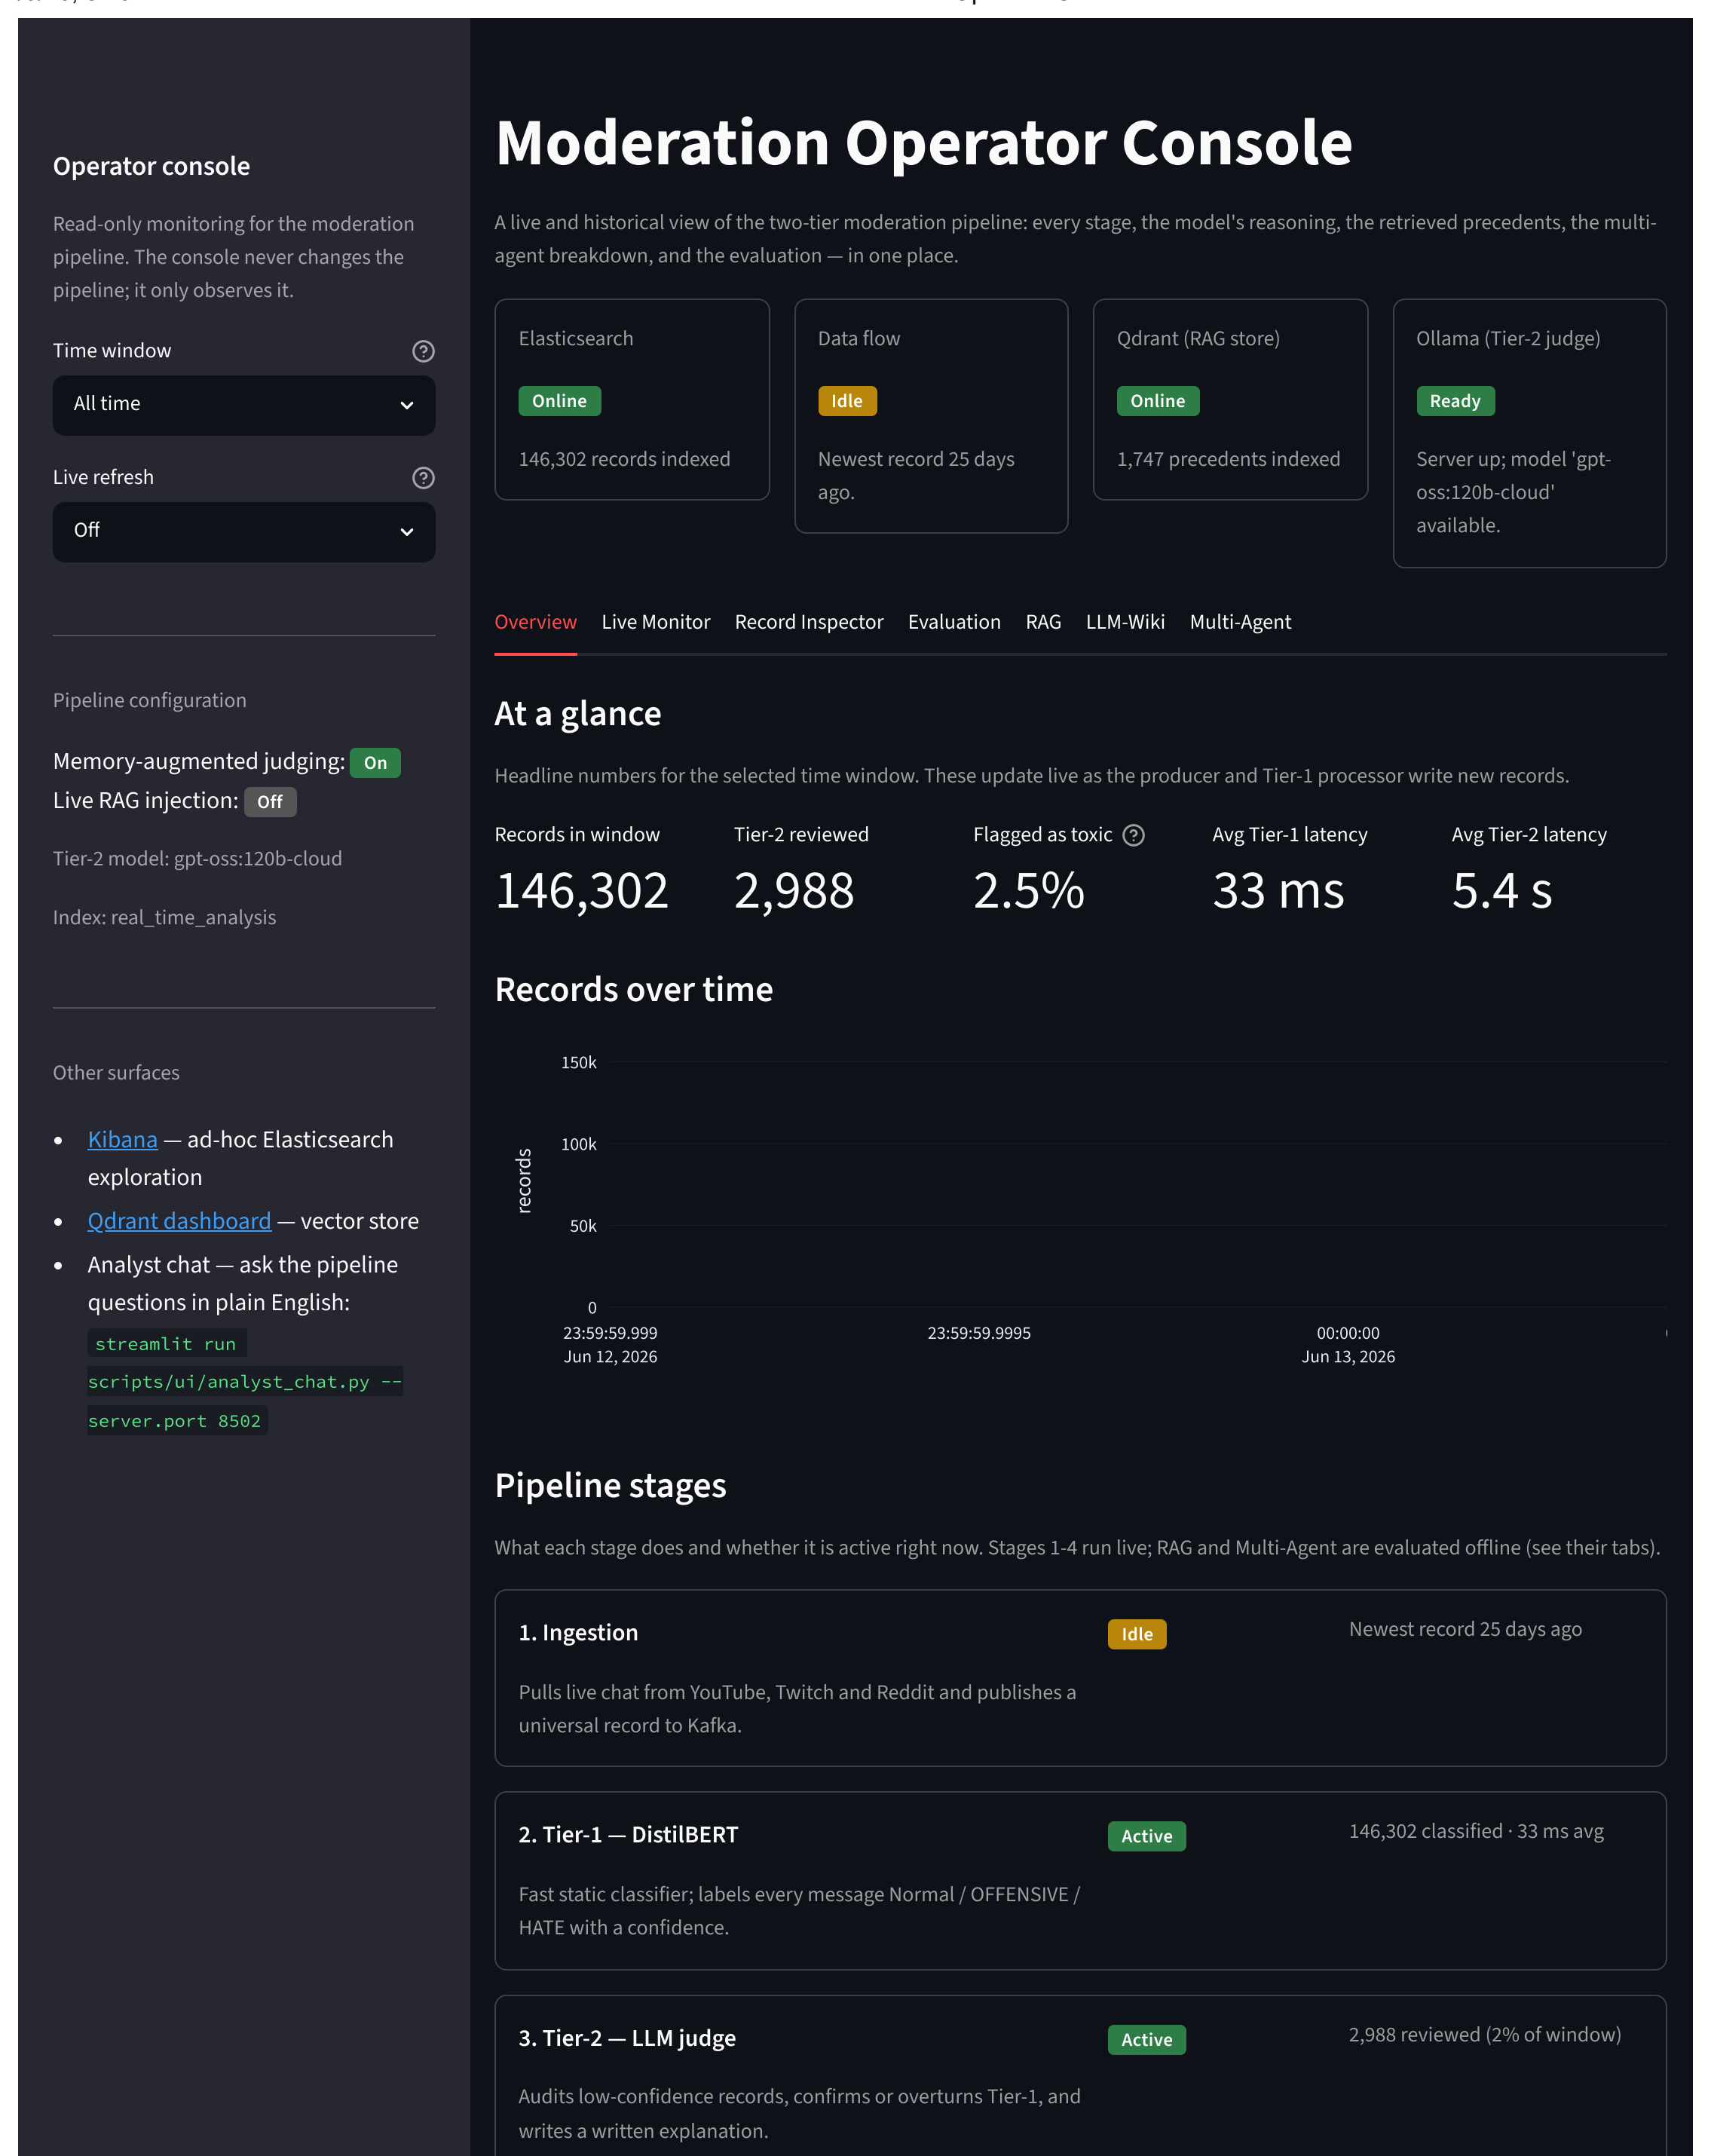
\includegraphics[width=1.5\linewidth,height=0.85\textheight,keepaspectratio]{figures/dashboard_overview.png}
\caption{The operator dashboard (Overview tab), built in Streamlit: the live status strip, the at-a-glance headline numbers, and the per-stage pipeline view.}
\end{figure}

\begin{figure}[H]
\centering
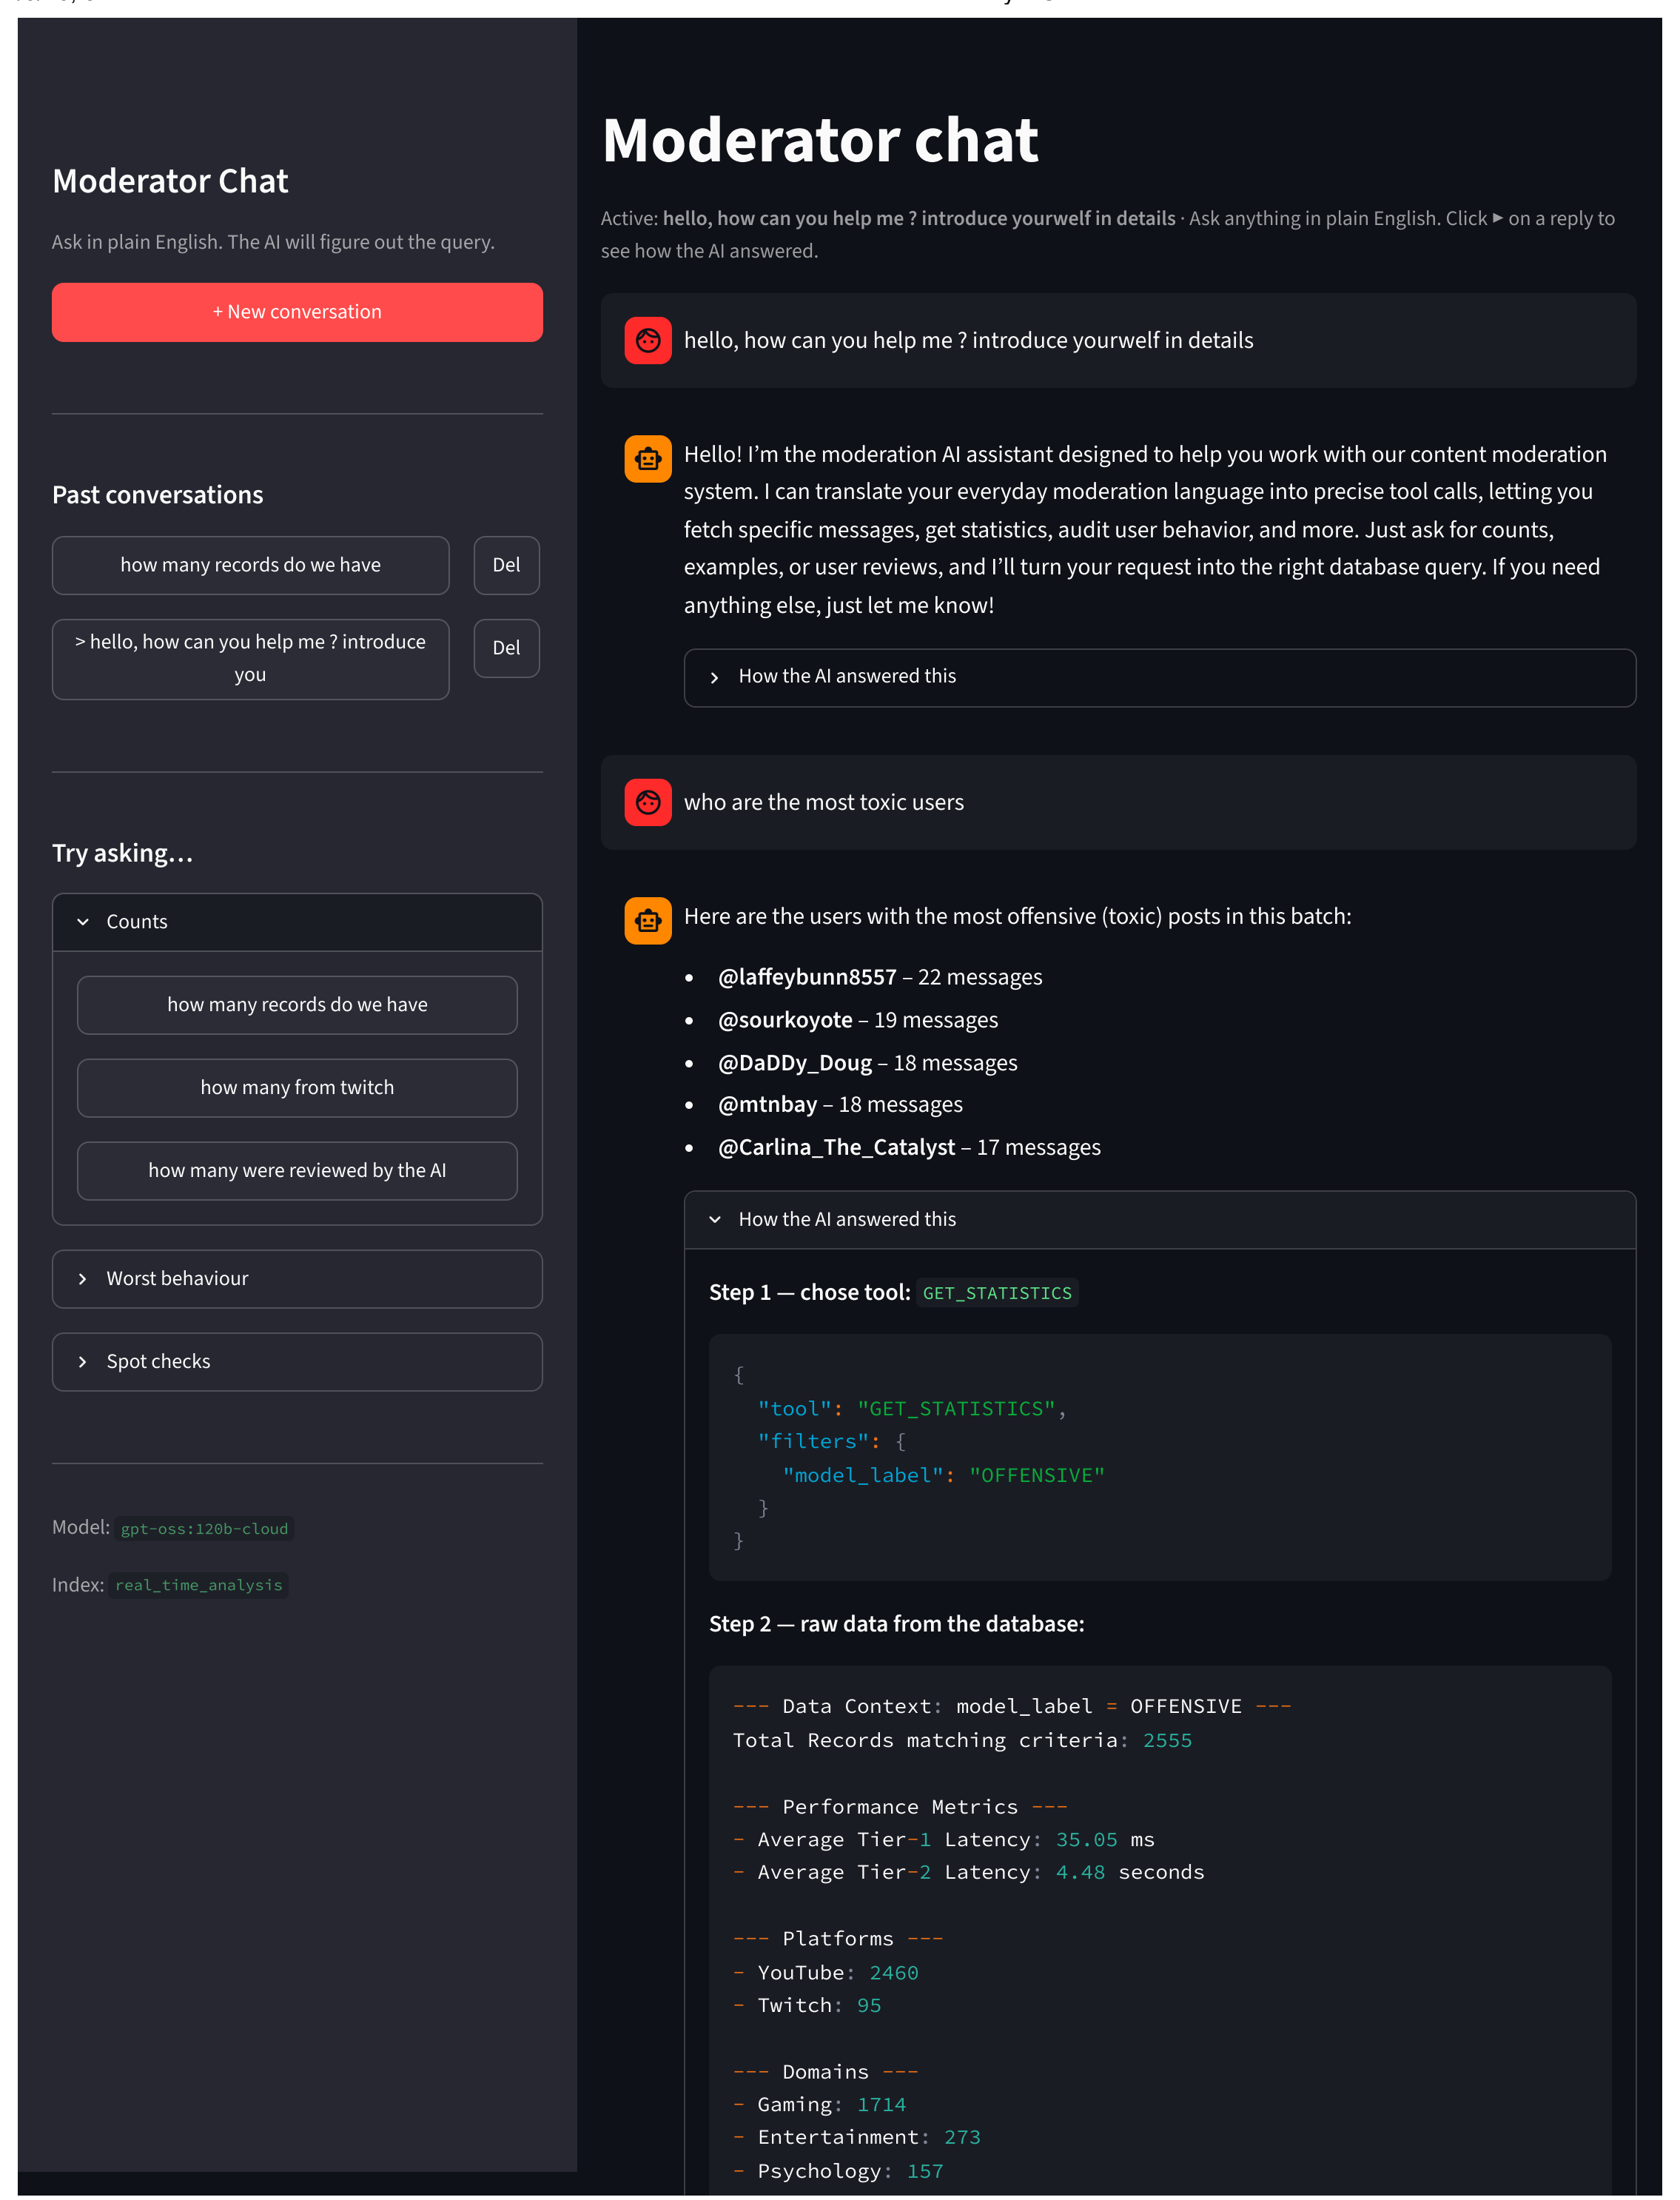
\includegraphics[width=1.5\linewidth,height=0.85\textheight,keepaspectratio]{figures/analyst_chat.png}
\caption{The natural-language analyst console: a plain-English question (``who are the most toxic users'') is turned into a tool call, and the expandable ``How the AI answered this'' panel shows the chosen tool and the raw data behind the reply.}
\end{figure}

\section{The Universal Schema}\label{the-universal-schema}

Two contracts hold the pipeline together. Keeping them apart was deliberate.

The first is the \textbf{Universal Kafka payload}, the shape every producer must emit and the processor consumes. It carries the message text, the source platform, the Context Agent's fields (domain, sub-genre, strictness, and the reasoning behind them), and a nested bag of platform-specific metadata: message and thread identifiers, author, role flags. Its one job is to guarantee the processor never breaks on a missing field. Anything a platform wants to add goes in the metadata bag, and nothing downstream has to care.

The second is the \textbf{Elasticsearch document}, which is what the processor writes and what the dashboards and agents read. It begins as the Tier-1 record, with identity, source context, author, and the DistilBERT prediction and its latency. Tier-2 then \emph{overlays} its verdict and explanation on top, and as the thesis progresses each variant gets its own named slot: memory, retrieval, multi-agent. Those slots never overwrite each other. That is what keeps the original baseline numbers reproducible no matter how many reasoning strategies get layered on afterwards.

Here i used two schemas instead of one shared object,Because producers and analysts care about genuinely different things. A producer has no business knowing a Tier-2 memory field exists. A dashboard should see exactly what is in storage and never an ingestion-side internal leaking through. The seam between the two is precisely where Tier-1 hands off to everything that follows.

\section{Deployment and reproducibility}\label{deployment-and-reproducibility}

The entire infrastructure is defined in a single \texttt{docker-compose} file, so anyone can stand it up and try it in their own environment.

Following the comparisons above, the final set of tools is: Kafka and Zookeeper for the broker, a Spark master and worker for distributed compute, Elasticsearch and Kibana for storage and visualisation, and Qdrant for vectors, all on one private network with persistent volumes.

The LLM is the only component outside that stack, reached through Ollama. A 120-billion-parameter judge does not fit the modest 4\,GB GPU the rest of the system was designed around, so the experiments reported here run \texttt{gpt-oss:120b} on Ollama's hosted endpoint. The same interface also serves a fully local model with no change to the pipeline, and that matters for more than convenience. A local open-weight model such as \texttt{dolphin-llama3} is not bound by the content policies that hosted providers apply, and those policies are a real obstacle in this field: a moderation system has to reason about the very language a general-purpose assistant is trained to refuse. Moving the judge on-premise, on adequate hardware, is therefore a one-line configuration change rather than a redesign, and it buys both privacy and freedom from a refusal that would otherwise arrive mid-evaluation.
